\section{Mission frontend}

Pendant mon alternance liée au projet Pipeline Documentaire, j'ai également travaillé sur une mission frontend. Ma responsabilité était de transformer la page d'importation des fichiers de transactions de carburant dans le projet Gestion de parc. Cette transformation a impliqué les modifications suivantes :

\begin{itemize}
    \item Réorganisation de l'emplacement du bouton de téléchargement de fichiers et du bouton d'importation.
    \item Ajout d'un bouton pour afficher une fenêtre modale.
    \item Intégration de la fenêtre modale affichant un guide sur la manière de télécharger les fichiers de transaction de carburant à partir des sites web des différents prestataires.
    \item Adaptation de la page afin qu'elle communique avec le Pipeline Documentaire au lieu de l'ancienne API pour certains types de fichiers de transactions de carburant.
    \item Affichage de messages sur l'état de l'importation tout au long du processus.
\end{itemize}

La raison derrière cette mission était que selon les retours des utilisateurs, la page d'origine dédiée à l'importation des fichiers de transactions de carburant manquait de convivialité et ne répondait pas aux attentes de leur expérience. Ils ne savaient souvent pas où obtenir les fichiers de transactions de carburant, et lorsqu'ils importaient un fichier via la page, ils ne savaient pas si l'importation avait réussi ou échoué, et en cas d'échec, ils ne comprenaient pas pourquoi. Cela peut être vu sur la version originale de la page d'importation (Figure~\ref{fig:original-import-page}).

\begin{figure}[ht]
    \centering
    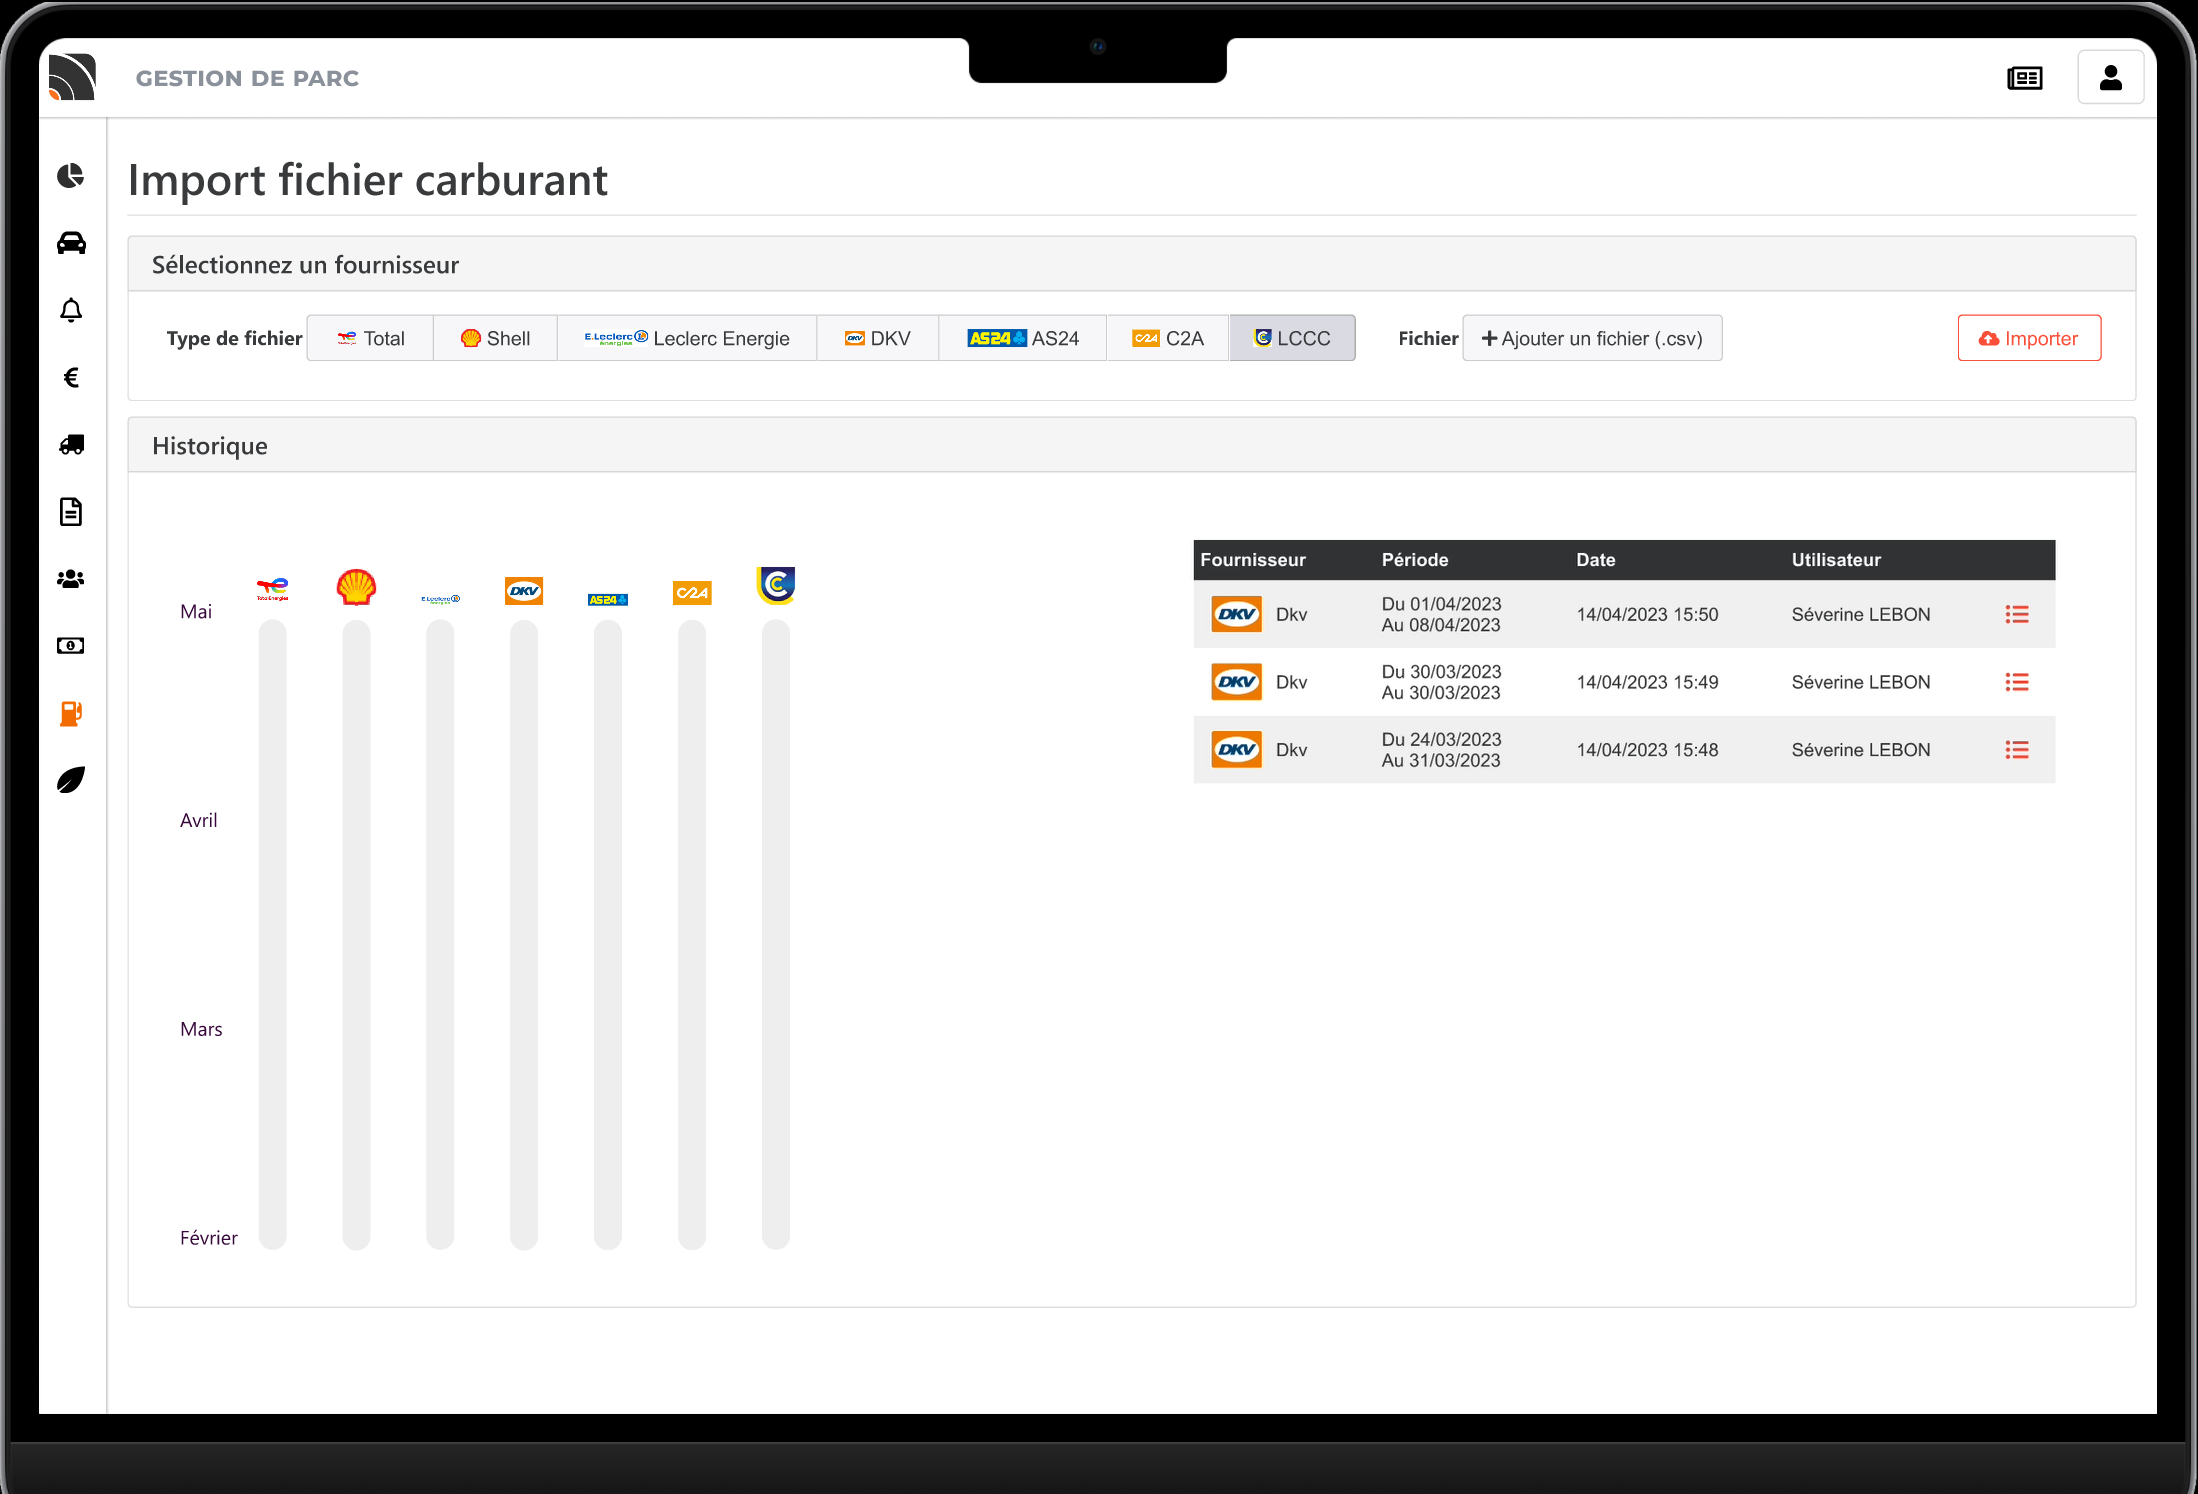
\includegraphics[width=0.73\textwidth]{img/frontend-maquettage-original}
    \caption{La version originale de la page d'importation des fichiers de transaction de carburant.}
    \label{fig:original-import-page}
\end{figure}

Pour accomplir cette mission, j'ai tout d'abord dû créer une maquette de la nouvelle apparence de la page, en tenant compte des exigences. Après quelques ajustements issus de discussions avec le propriétaire du produit, la version finale de la maquette a été approuvée, me permettant ainsi de débuter sa mise en œuvre. Dans cette section, je vais présenter les détails de la maquette que j'ai élaboré, ainsi que la mise en œuvre technique des modifications relatives à l'importation du fichier de transactions de carburant.

\subsection{Maquettage}

Les figures suivantes illustrent différents aspects de la maquette : la réorganisation des boutons et l'ajout du bouton \foreignquote{french}{Guide de téléchargement} (Figure~\ref{fig:frontend-maquettage-total-buttons}), l'intégration de la fenêtre modale (Figure~\ref{fig:frontend-maquettage-total-modal}), ainsi que la présentation des retours à l'utilisateur en cas de succès ou d'erreur et leur séquence (Figure~\ref{fig:frontend-maquettage-total-file-sent}, Figure~\ref{fig:frontend-maquettage-feedbacks}). J'ai créé cette maquette interactive dans Figma et elle est disponibles sur le lien \url{https://figma.fun/kIw9mt}.

\begin{figure}[ht]
    \centering
    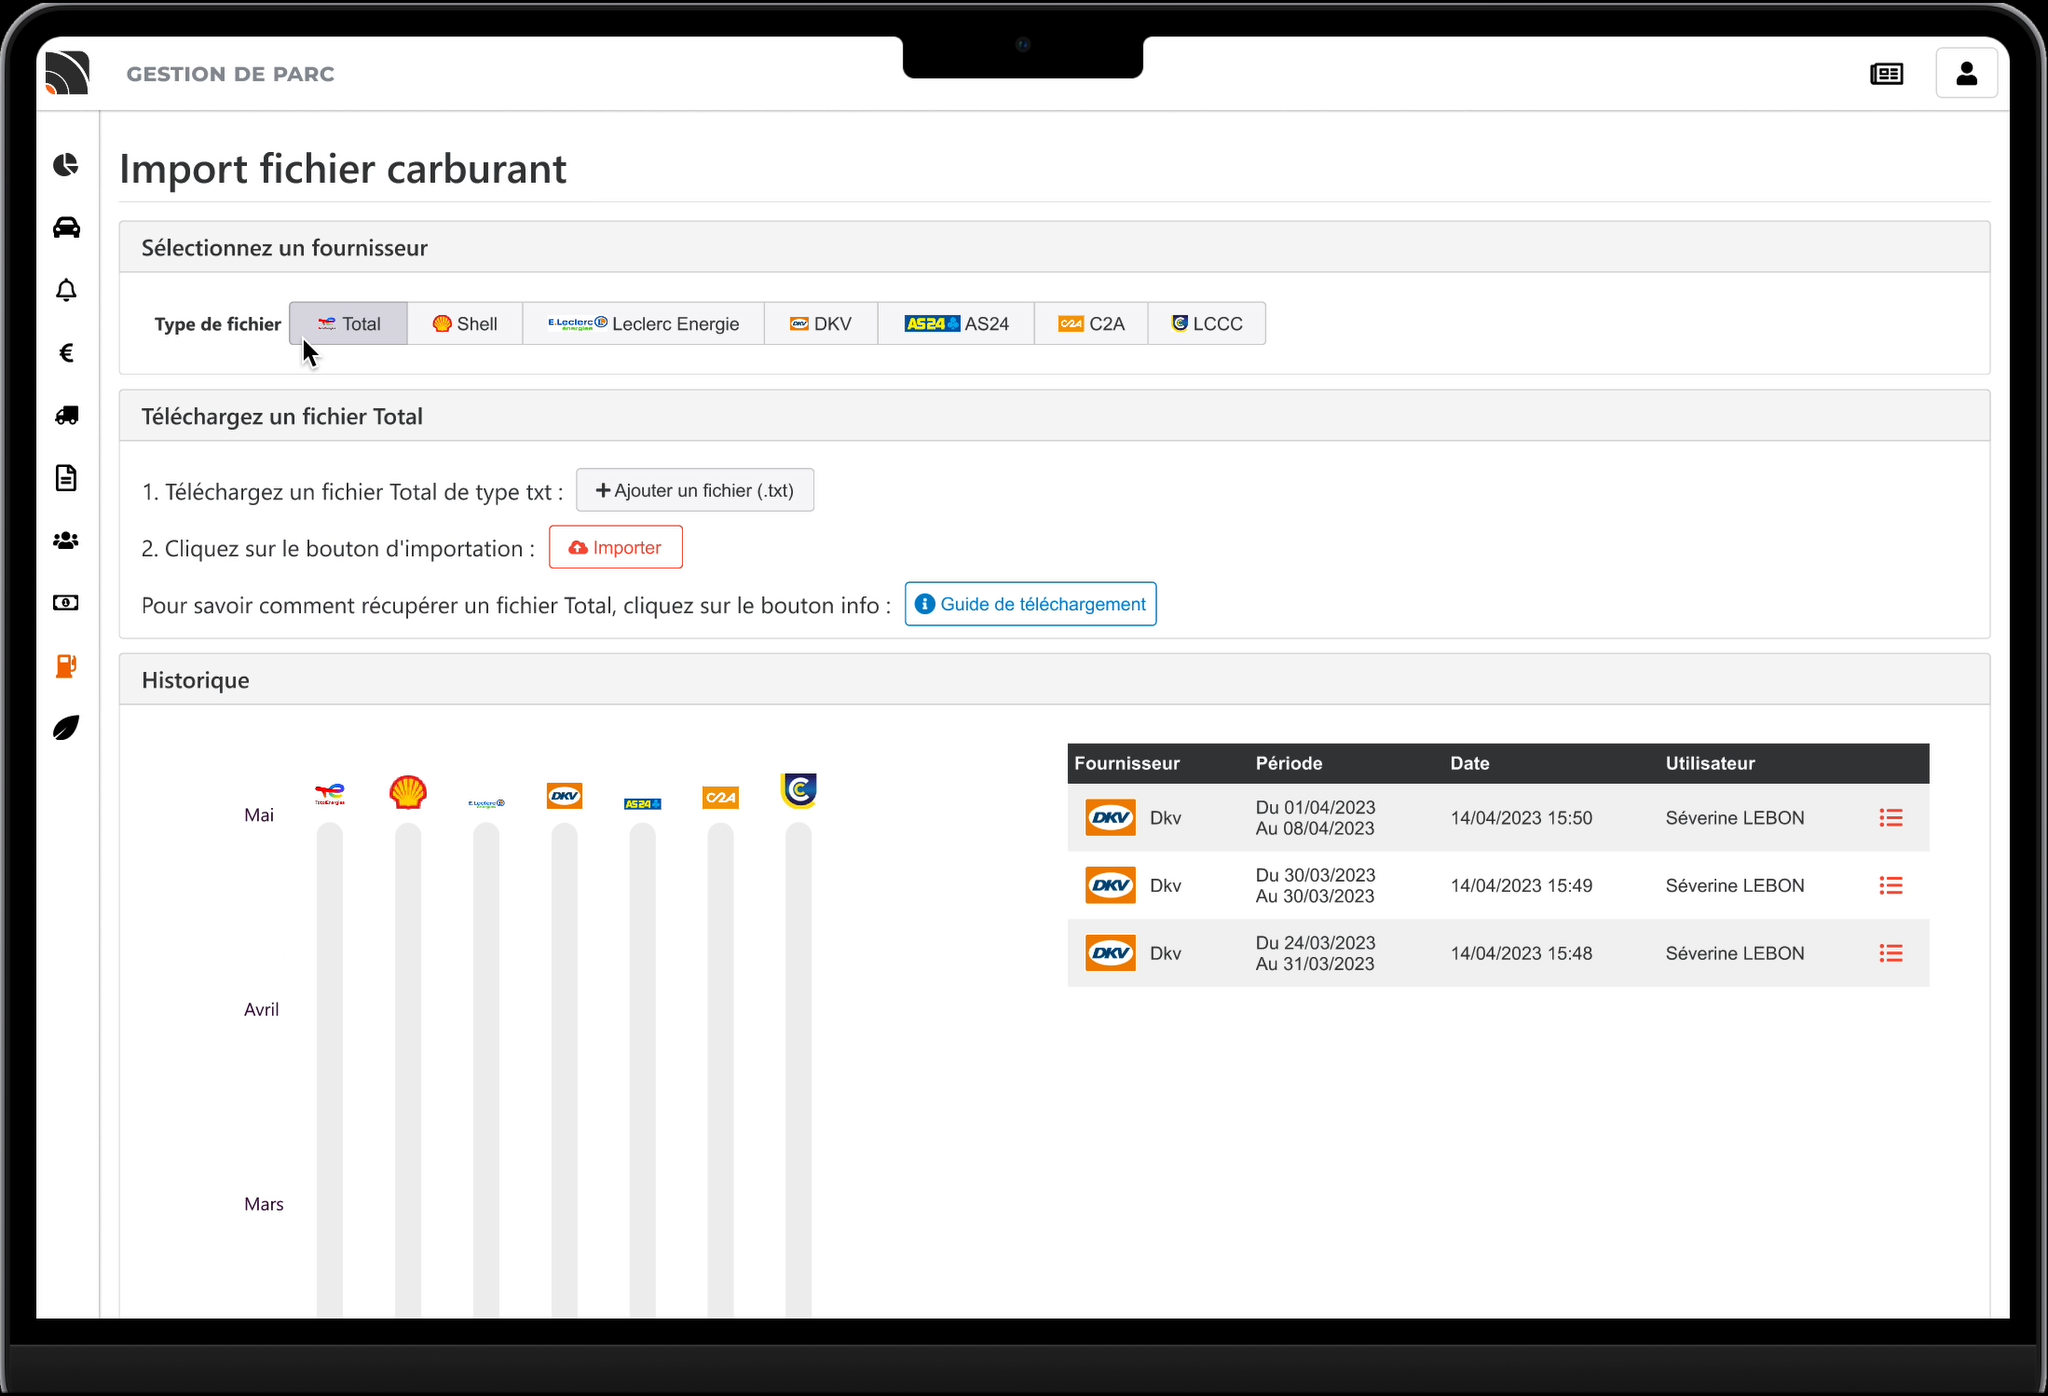
\includegraphics[width=0.73\textwidth]{img/frontend-maquettage-total-buttons}
    \caption{La maquette de la page d'importation des fichiers de transaction de carburant avec le placement réorganisé des boutons et le bouton Guide de téléchargement ajouté.}
    \label{fig:frontend-maquettage-total-buttons}
\end{figure}

\begin{figure}[ht]
    \centering
    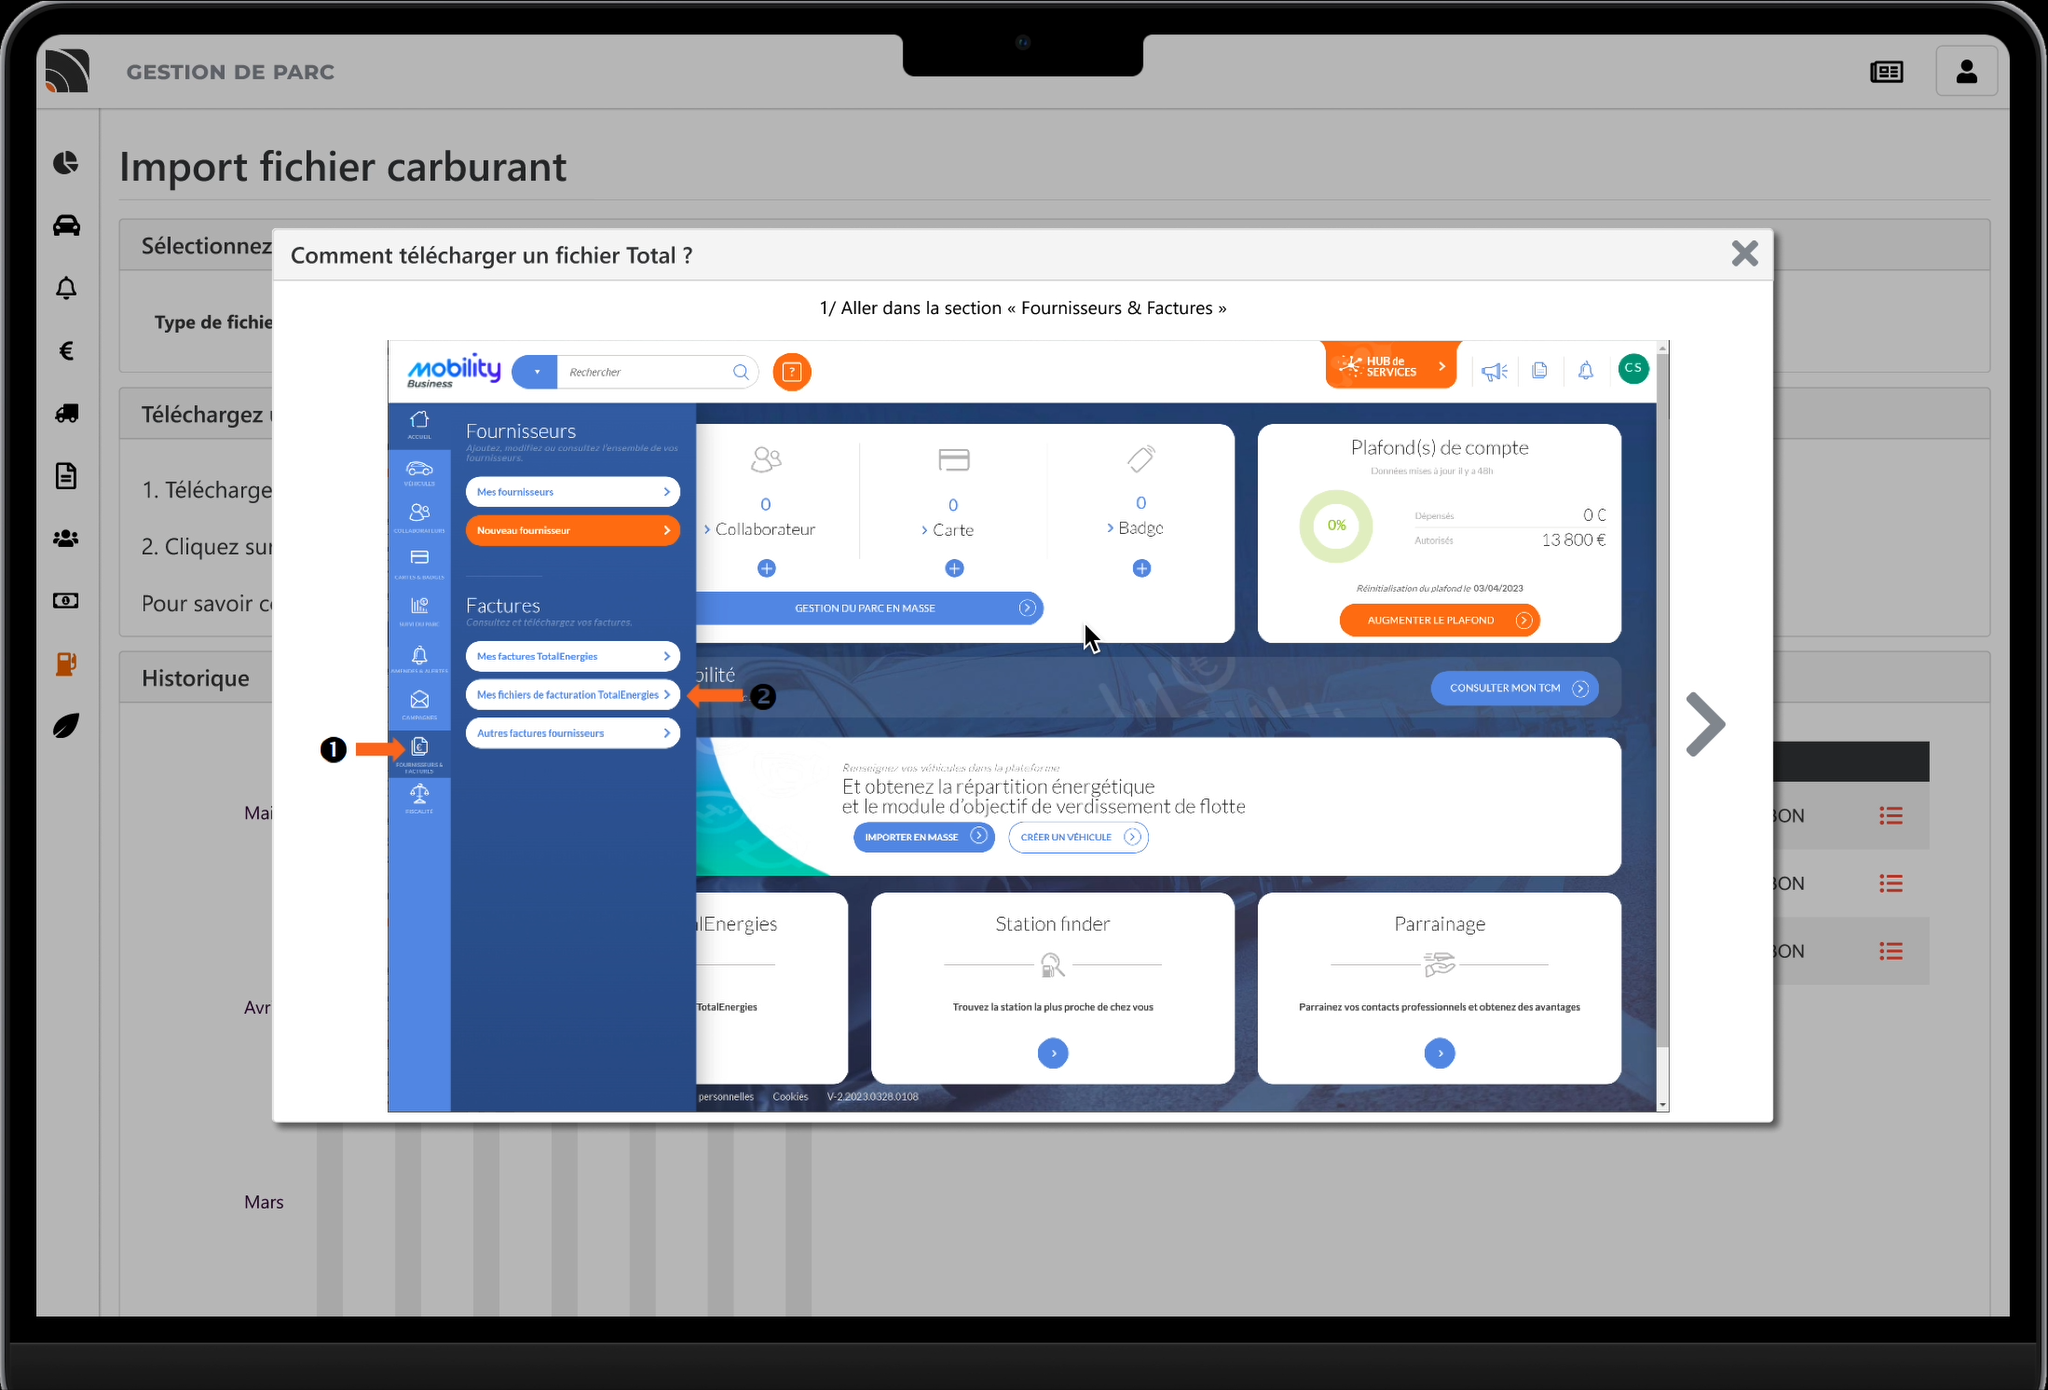
\includegraphics[width=\textwidth]{img/frontend-maquettage-total-modal}
    \caption{La maquette de la page d'importation des fichiers de transaction de carburant avec la fenêtre modale.}
    \label{fig:frontend-maquettage-total-modal}
\end{figure}

\begin{figure}[ht]
    \centering
    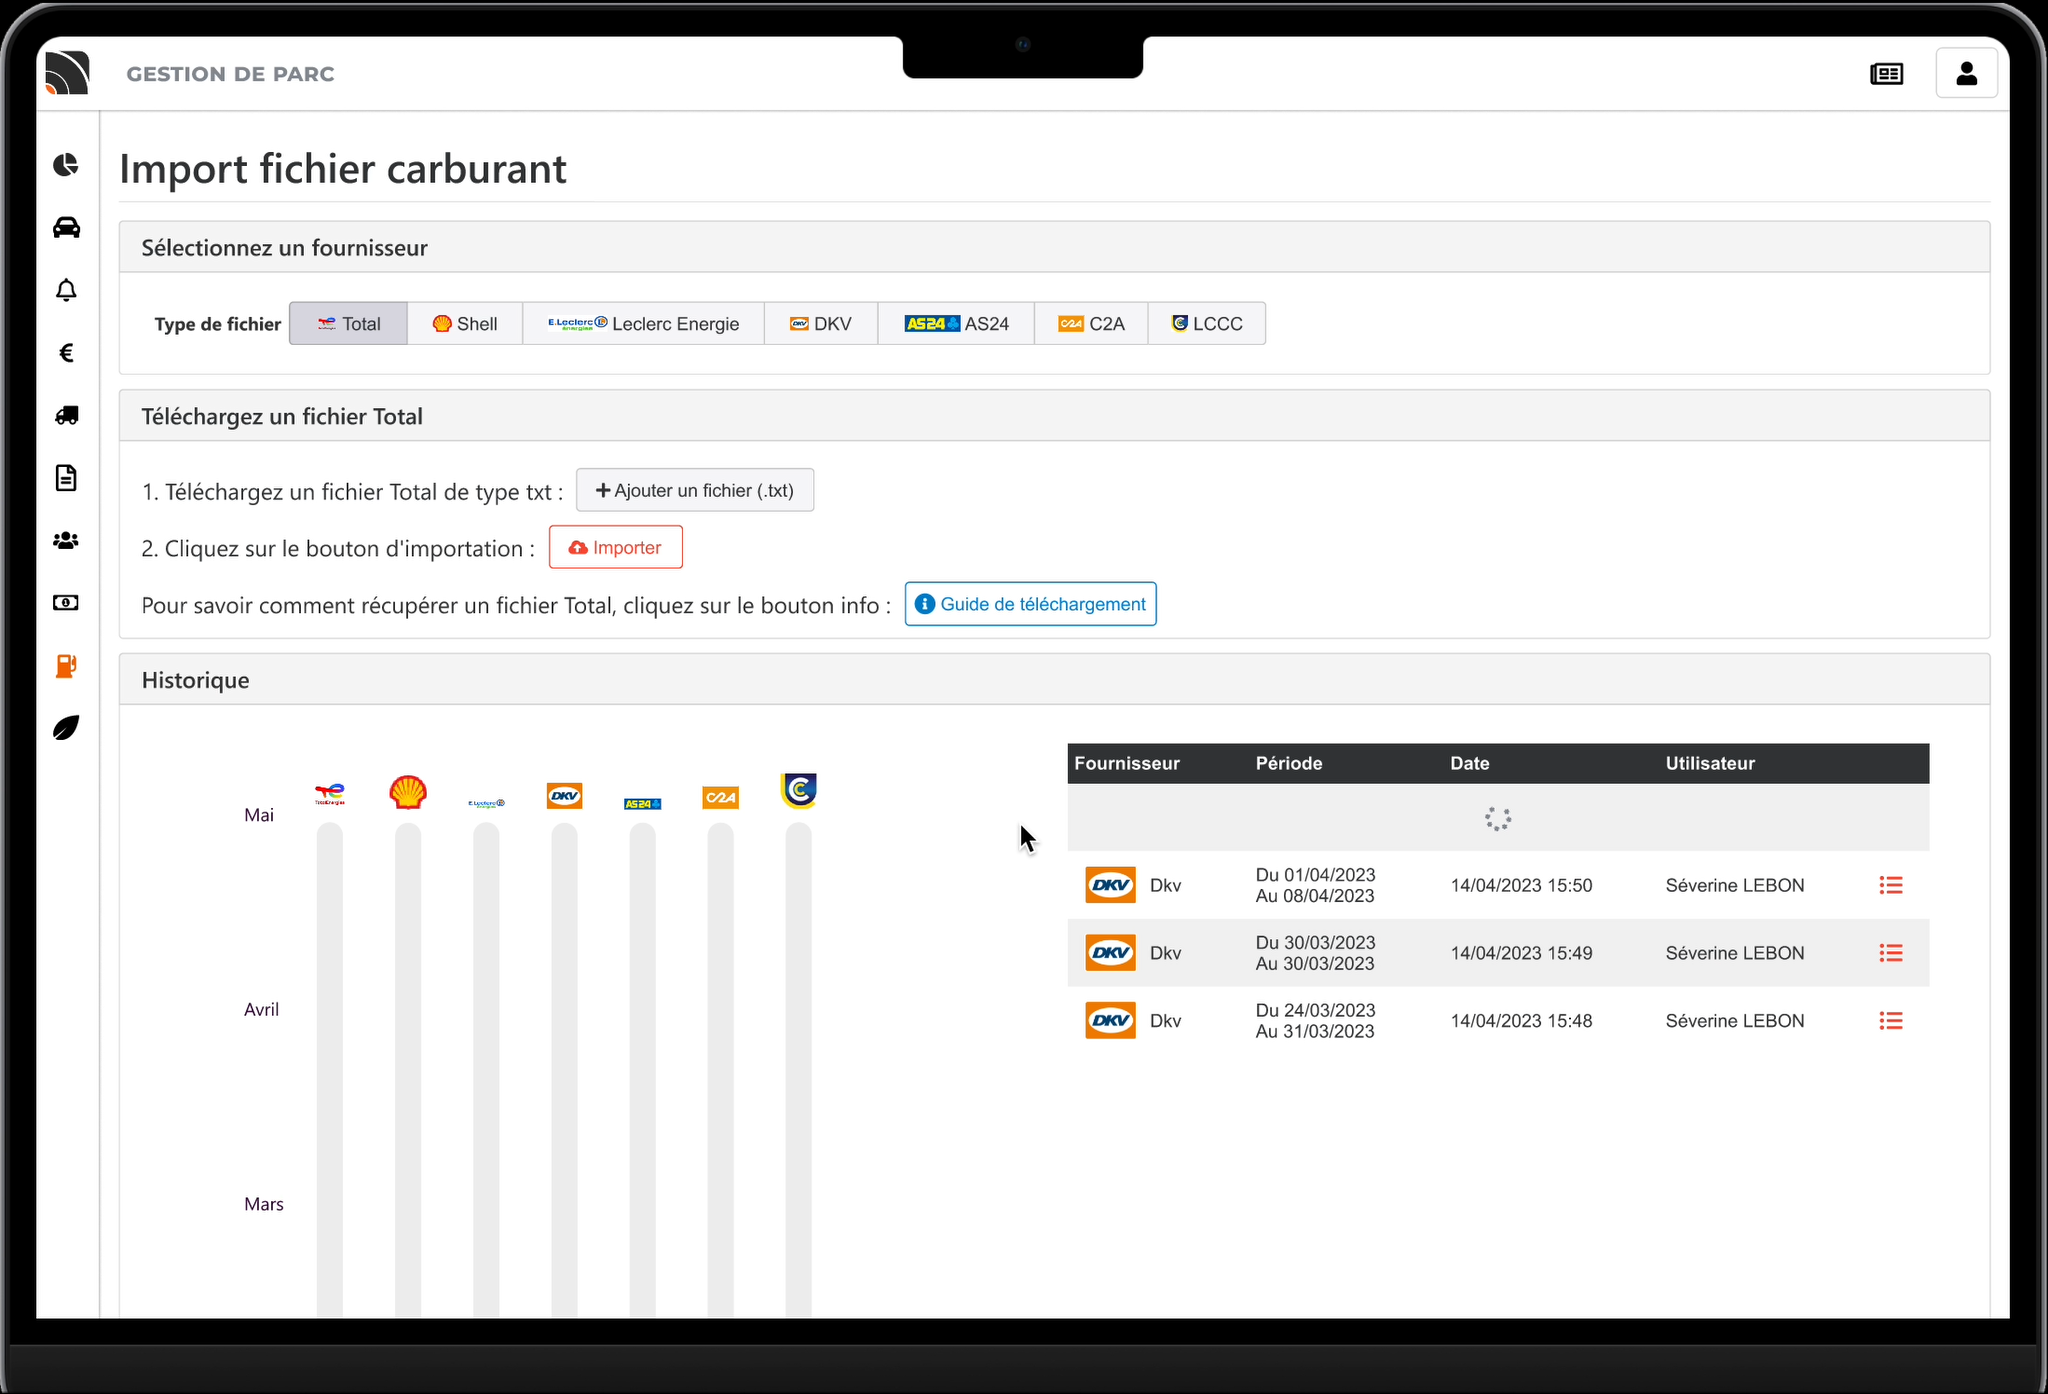
\includegraphics[width=\textwidth]{img/frontend-maquettage-total-file-sent}
    \caption{La maquette de la page d'importation des fichiers de transaction de carburant. Après avoir cliqué sur le bouton d'importation, l'utilisateur reçoit un retour indiquant que le fichier a été envoyé pour être importé.}
    \label{fig:frontend-maquettage-total-file-sent}
\end{figure}

\begin{figure}[ht]
    \centering
    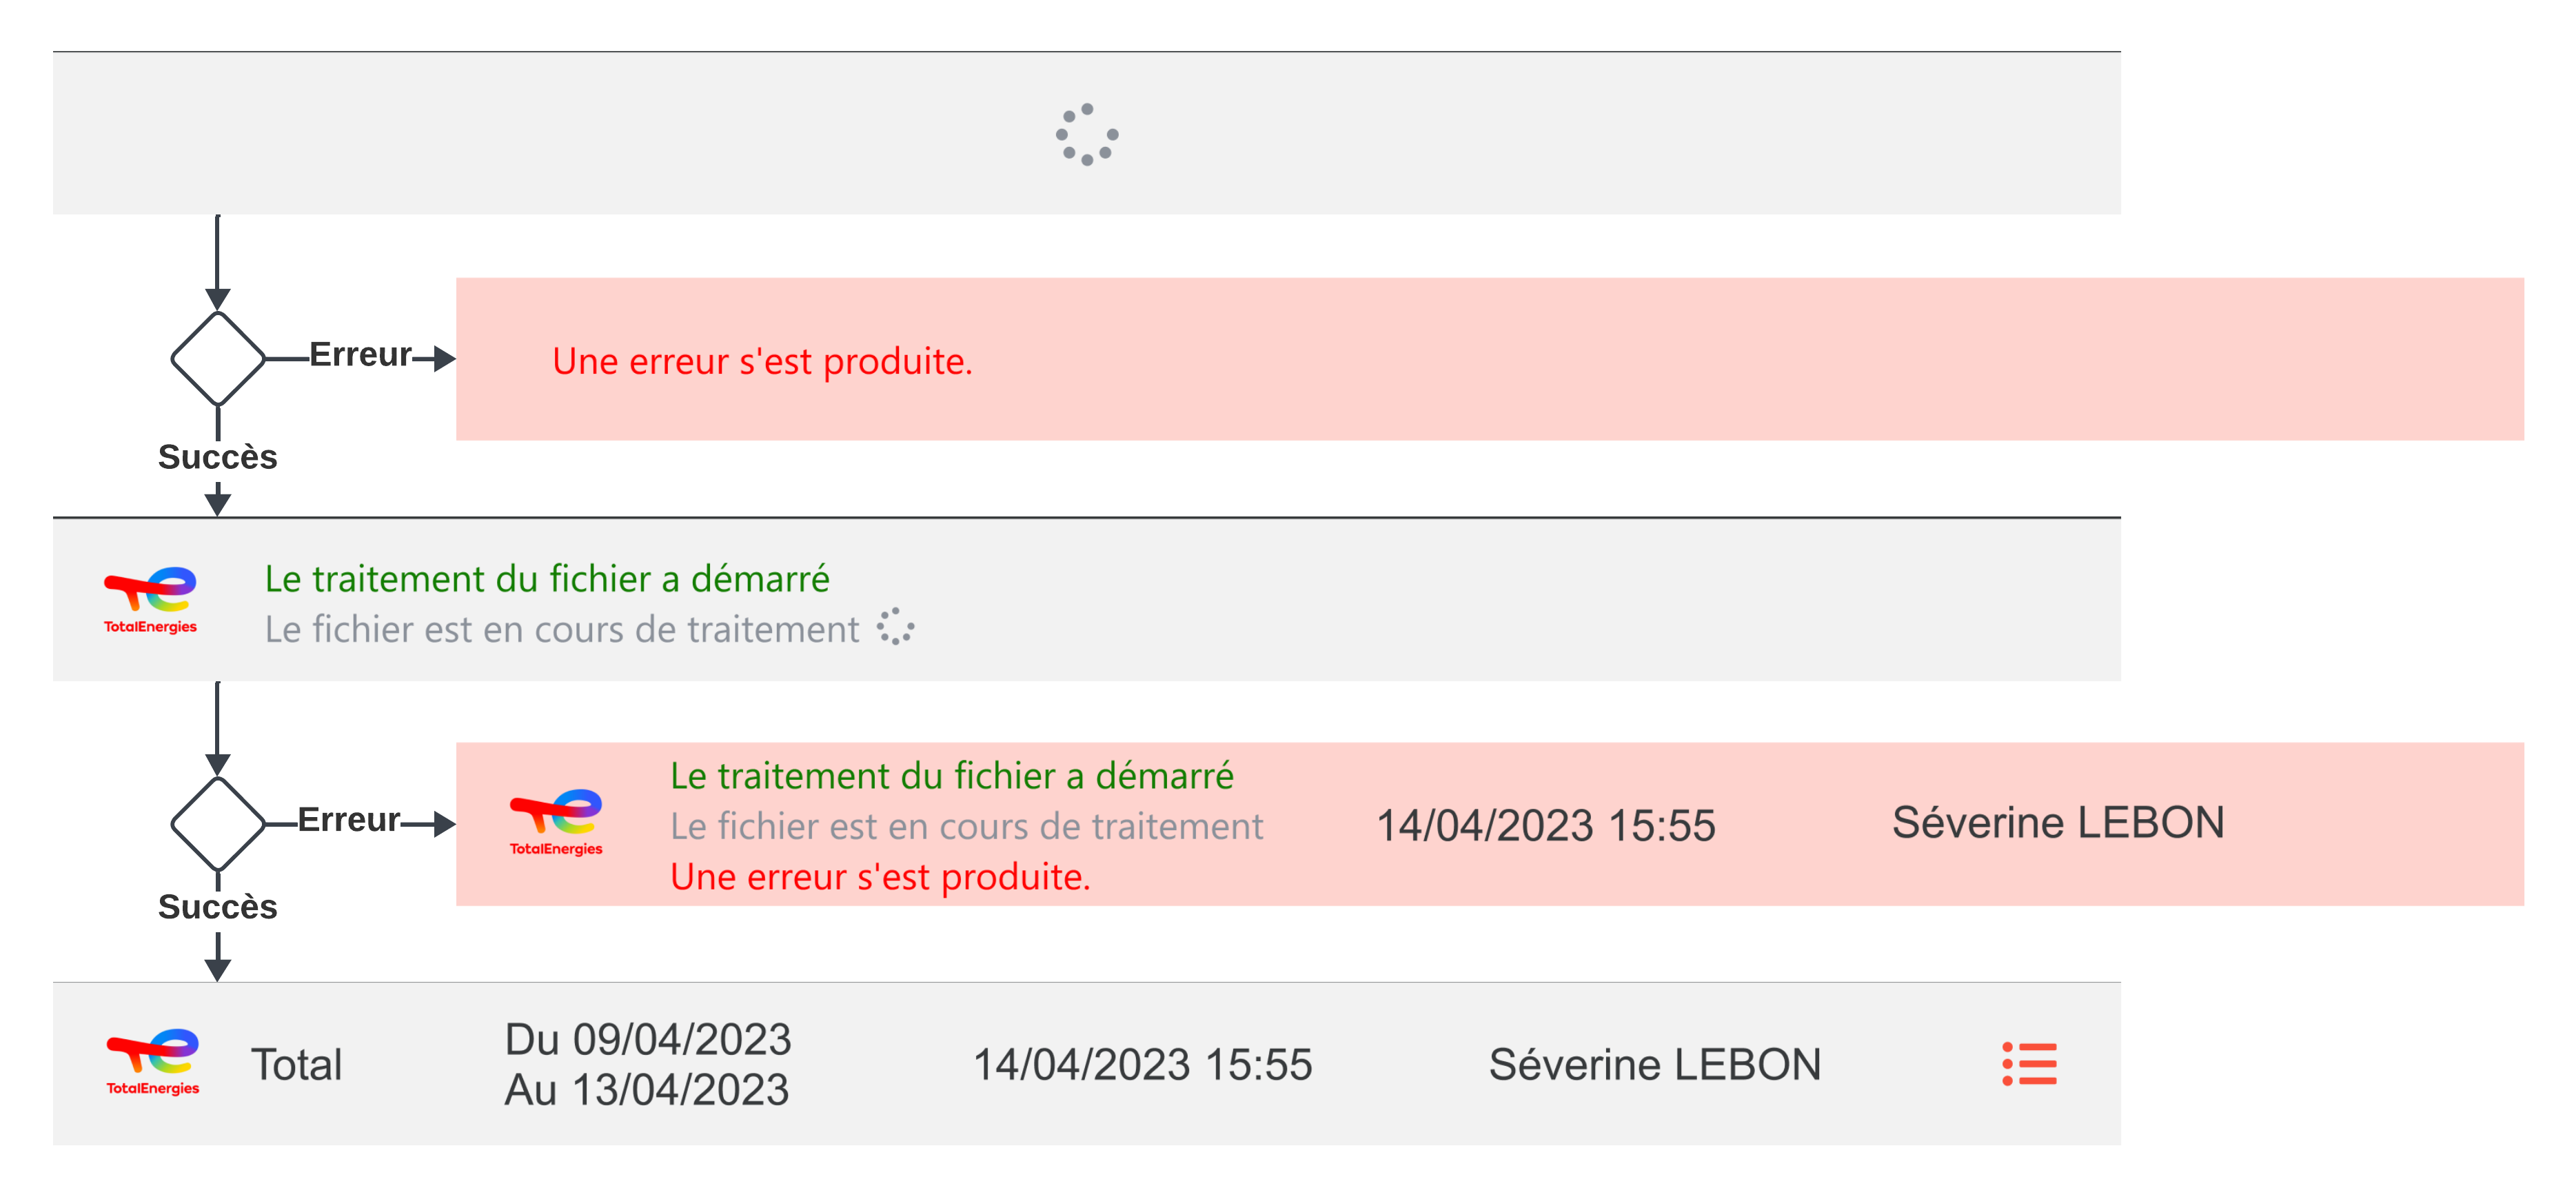
\includegraphics[width=\textwidth]{img/feedbacks}
    \caption{Série de retours à l'utilisateur sur l'état de l'importation du fichier.}
    \label{fig:frontend-maquettage-feedbacks}
\end{figure}

\subsection{Développement frontend}

